
\section{Remover}
\label{subs:remover}

%\begin{figure}[h]
%\centering
%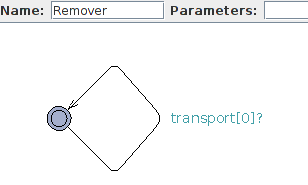
\includegraphics[width=0.6\textwidth]{firstremover.png}
%\caption{The model of the remover template}
%\label{fig:firstremover}
%\end{figure}

%The \emph{remover template} is not very complex, and can be seen in \cref{fig:firstremover}. It continously tries to synchronise on the \emph{transport} channel 0, in order to remove a recipe from the factory. The factory modules each have their own \emph{transport} channel, given by their ID, which is 1-indexed. Thus, a \emph{transport} on channel 0 does not pass the recipe to a module, but instead to the remover. If we want to remove a recipe, when it is passed on from a specific module, we simply set one of the IDs in the module’s next array to 0. Removing a recipe from a factory is especially beneficial in circular setups, as a finished recipe may otherwise be passed around indefinitely. This may unnecessarily decrease factory throughput. By removing recipes. We also decrease the state space that needs to be searched by the model checker.
